\documentclass[16pt]{beamer}

% 字体设置
\usepackage{fontspec}
\setsansfont{Times New Roman}

% 图片和颜色
\usepackage{graphicx}
\usepackage{caption}
\usepackage{xcolor}
\usepackage{amsmath} % 数学符号
\usepackage{booktabs} % 更漂亮的表格

% Beamer 主题
\usetheme{Madrid}

% 自定义调色
\definecolor{MainBlue}{cmyk}{1,0.7,0,0} % C=100, M=70
\definecolor{SecondaryCyan}{cmyk}{1,0,0,0} % C=100, M=0

\setbeamercolor{structure}{fg=MainBlue}
\setbeamercolor{frametitle}{bg=MainBlue!20!white, fg=MainBlue}
\setbeamercolor{itemize item}{fg=MainBlue}

% 插入 logo
\pgfdeclareimage[height=1.3cm]{logo}{University_of_International_Business_and_Economics_LOGO.png}
\logo{\pgfuseimage{logo}}

% 目录自动出现
\AtBeginSection[]
{
  \begin{frame}<beamer>
    \frametitle{Outline}
    \tableofcontents[currentsection]
  \end{frame}
}

% 标题等信息
\title{UIBE Beamer Template}
\author{Mochiao Chen\thanks{mochiaochen@gmail.com}}
\date{\today}

\begin{document}

% 封面
\begin{frame}
  \titlepage
\end{frame}

% 目录
\begin{frame}
  \frametitle{Outline}
  \tableofcontents
\end{frame}

% 第一节:段落 + 分点
\section{Introduction}
\begin{frame}
  \frametitle{Introduction}
  \textbf{This is a normal paragraph for demonstration.}
  
  Beamer allows you to present your ideas clearly and professionally.
  You can mix normal text with bullet points:
  
  \begin{itemize}
    \item First key point
    \item Second key point
    \item Third key point
  \end{itemize}
\end{frame}

% 第二节:数学公式
\section{Mathematical Formula}
\begin{frame}
  \frametitle{Mathematical Example}
  
  Here is an inline formula: \( E = mc^2 \)

  And a displayed equation:
  \[
    \int_{-\infty}^{\infty} e^{-x^2} dx = \sqrt{\pi}
  \]

  Or a numbered equation:
  \begin{equation}
    f(x) = ax^2 + bx + c
  \end{equation}
\end{frame}

% 第三节:表格
\section{Table Example}
\begin{frame}
  \frametitle{Sample Table}
  
  \begin{table}[h!]
    \centering
    \caption{Example Data Table}
    \begin{tabular}{lccc}
      \toprule
      Item & Value 1 & Value 2 & Value 3 \\
      \midrule
      A & 10 & 20 & 30 \\
      B & 40 & 50 & 60 \\
      C & 70 & 80 & 90 \\
      \bottomrule
    \end{tabular}
  \end{table}
\end{frame}

% 第四节:插入图片
\section{Image Example}
\begin{frame}
  \frametitle{Sample Image}

  Below is a sample image inserted:

  \begin{figure}[h!]
    \centering
    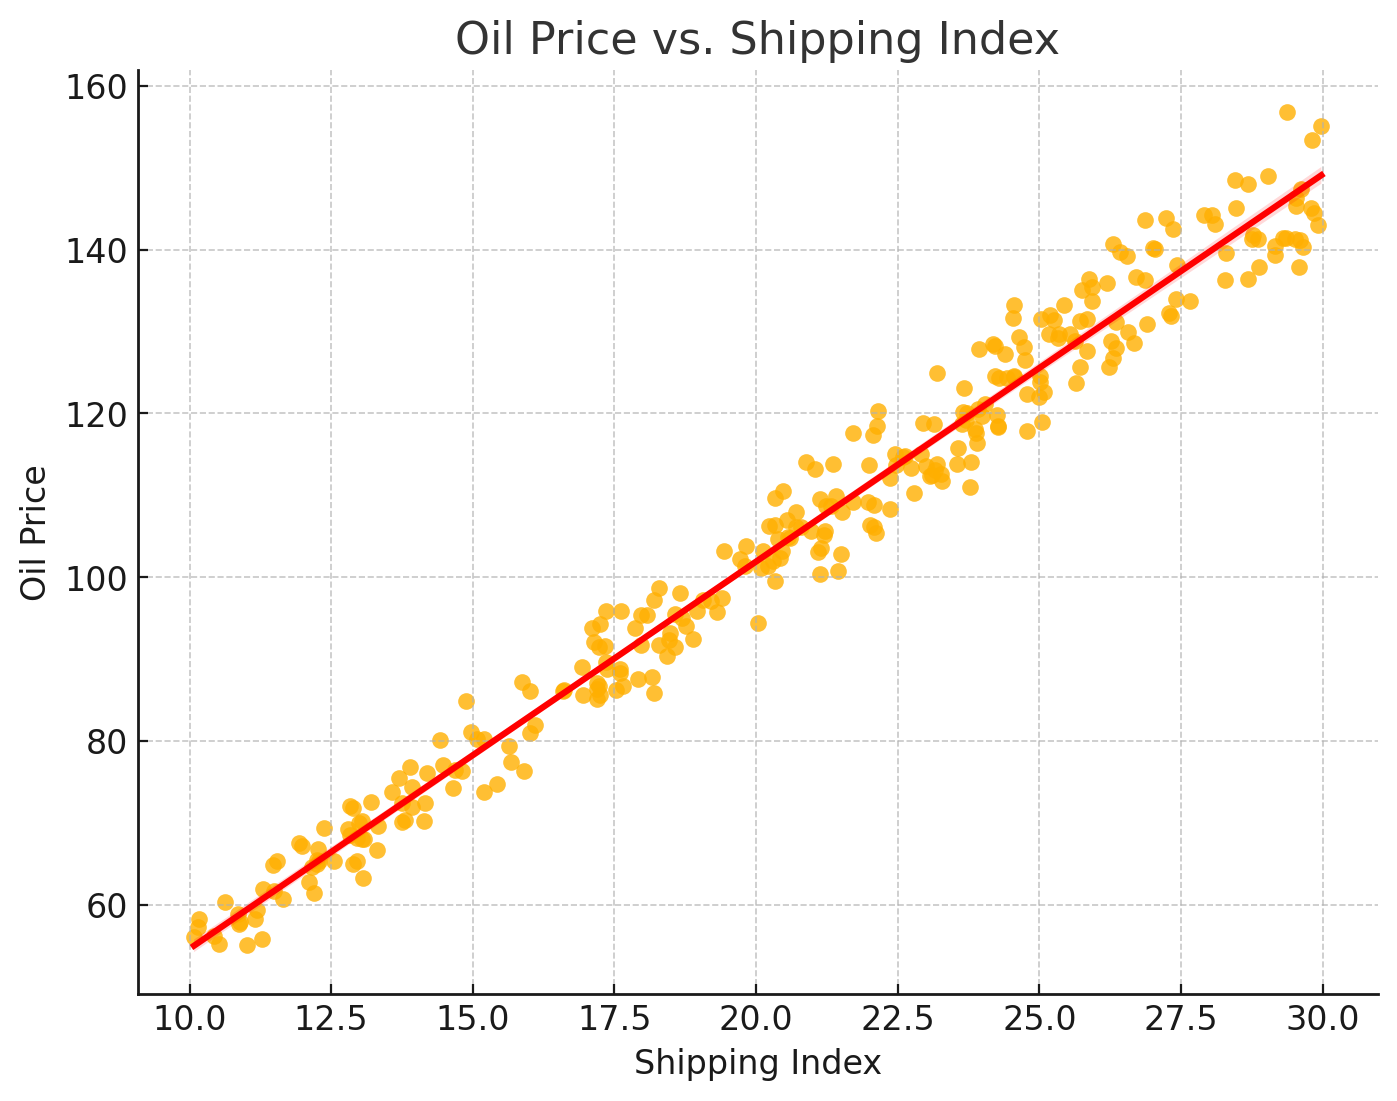
\includegraphics[width=0.5\textwidth]{Oil_price_vs_Shipping_index.png} % 替换为你的图片名
    \caption{Oil Price vs Shipping Index}
  \end{figure}

  Remember to keep your images in the same directory or provide a path.
\end{frame}

% 结束
\begin{frame}
  \centering
  \Huge Thank You!
\end{frame}

\end{document}
